%Exemplo de capitulo

\chapter{Redes Neurais Convolucionais}

Rede neural artificial (\sigla{ANN}{\emph{Artificial Neural Network},
rede neural artificial}, do inglês, \emph{Artificial Neural Network}) é um modelo computacional inspirado na forma com
que o cérebro resolve problemas \cite{gilbert2000build}. Este modelo possui
unidades, denominadas neurônios, que possuem um valor que é calculado como uma
função do valor de outros neurônios.

\begin{figure}[!htb]
	\centering
	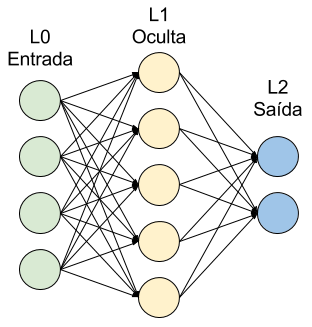
\includegraphics[scale=0.7]{ex_fcnn.png}
	\caption[Exemplo de rede neural totalmente conectada]{
		Exemplo de rede neural totalmente conectada (autoria própria).}
	\label{fig:ex_fcnn}
\end{figure}

Alguns neurônios especiais, denominados “entradas” possuem um valor obtido de
fora do sistema. Estes são especiais porque são os únicos cujos valores não são
calculados. O valor de alguns dos neurônios de uma rede neural artificial podem
afetar sistemas externos a ela. Por isso são designados “saídas”. Neurônios que
não são de entrada ou de saída são chamados “ocultos”. A figura
\ref{fig:ex_fcnn} ilustra uma rede neural simples com os três tipos de
neurônios.

Neste capítulo será apresentada parte da teoria de redes neurais convolucionais
e não-convolucionais. Na seção \ref{sec:rnnc} apresentam-se as redes neurais
não-convolucionais, explorando algumas das suas propriedades matemáticas. Na
seção \ref{sec:rnc} será feita uma apresentação das redes convolucionais,
explorando vários de seus aspectos matemáticos e práticos.

\section{Redes Neurais Não-Convolucionais} \label{sec:rnnc}
As redes neurais artificiais são tipicamente organizadas em “camadas”, e a
escolha dos tipos de neurônio, juntamente com a forma com que os neurônios são
conectados, é denominada “topologia”. As redes são classificadas como
\emph{feedforward} (ou diretas) quando as conexões não formam ciclos ou
\emph{recurrent} (recorrentes) quando formam. Se
uma camada está conectada a todos os neurônios da camada anterior diz-se que a
camada é totalmente conectada.
A definição da função de transferência do neurônio é uma parte importante da
topologia das redes neurais. Um tipo muito comum de neurônio é definido por:

\begin{equation} \label{eq:non-conv-layer}
	v=A \left( \left( \sum_n w_n i_n \right) + b \right)
\end{equation}

Onde $v$ é o valor da saída do neurônio, $i_n$ é n-ésima entrada do neurônio,
$w_n$ é um escalar associado a esta entrada, denominado peso, e $b$ é um
escalar arbitrário, denominado \emph{bias}. Este último valor permite que um
neurônio produza valores não-nulos mesmo que a entrada seja nula. $A$ é uma
função denominada função de ativação do neurônio. Essa função pode ser usada
para tornar o neurônio não-linear, como no caso da tangente hiperbólica e da
função ReLu, ou linear retificada (ver figura \ref{fig:cap2_tanh_relu}). Os
pesos $w_n$ determinam a influência de cada entrada do neurônio.

\begin{figure}[!htb]
	\centering
	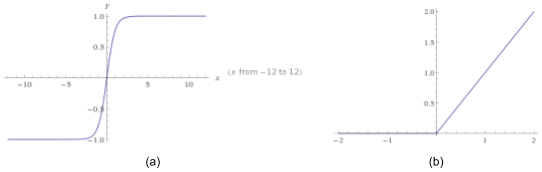
\includegraphics[scale=1]{cap2_tanh_relu.png}
	\caption[Comparação da tangente hiperbólica com a ReLu]{
		Comparação entre a função tangente hiperbólica e a Relu. Em (a) está a
		função tangente hiperbólica e em (b) está a função ReLu
		(autoria própria).}
	\label{fig:cap2_tanh_relu}
\end{figure}

A descrição de redes neurais com este tipo de neurônio e com topologia
totalmente conectada é especialmente conveniente. As três camadas
da rede neural ilustrada na figura \ref{fig:ex_fcnn} podem ser representadas
por matrizes:

\noindent\begin{minipage}{.333\linewidth}
	\begin{equation} \label{eq:l0}
		L0_{4 \times 1} =
			\begin{pmatrix}
				c_1 \\
				c_2 \\
				c_3 \\
				c_4
			\end{pmatrix}
	\end{equation}
\end{minipage}
\begin{minipage}{.333\linewidth}
	\begin{equation} \label{eq:l1}
		L1_{5 \times 1} =
			\begin{pmatrix}
				d_1 \\
				d_2 \\
				d_3 \\
				d_4 \\
				d_5
			\end{pmatrix}
	\end{equation}
\end{minipage}
\begin{minipage}{.333\linewidth}
	\begin{equation} \label{eq:l2}
		L2_{2 \times 1} =
			\begin{pmatrix}
				e_1 \\
				e_2
			\end{pmatrix}
	\end{equation}
\end{minipage}

Para calcular a primeira camada intermediária é preciso aplicar a equação
(\ref{eq:non-conv-layer}) cinco vezes, uma para cada neurônio. Porém, se
esta camada for totalmente conectada, e todos os neurônios usarem a
mesma função de transferência $A$, e a representação em matrizes estiver
sendo usada, o cálculo de todos os neurônios desta camada pode ser
realizado usando:

\begin{equation}
	L1_{5 \times 1}=A_V \left( W1_{5 \times 4} \times L0_{4 \times 1}
		+ B1_{5 \cdot 1} \right)
\end{equation}

Onde $A_V$ é uma versão vetorial da função de ativação resultante
da aplicação da função $A$ em cada um dos elementos do vetor.
Os pesos dos cinco neurônios, denominados $w_n$ na equação
\ref{eq:non-conv-layer} são aqui representados por uma única matriz
$W1_{5 \times 4}$, e os \emph{bias} dos cinco neurônios, $b$, são representados
por uma única matriz $B1_{5 \times 1}$. Da mesma forma, a camada de saída
pode ser calculada com:

\begin{equation}
	L2_{2 \times 1}=A_V \left( W2_{2 \times 5} \cdot L1_{5 \times 1}
		+ B2_{2 \times 1} \right)
\end{equation}

As matrizes $W$ e $B$ são os parâmetros que precisam ser aprendidos durante o
treinamento, e são denominados parâmetros treináveis. O número de parâmetros
de uma uma
rede neural é igual ao número de valores contidos em todas as matrizes de pesos
e \emph{bias}. Quanto maior o número de parâmetros, mais flexibilidade a rede
neural possui, porém mais lento é o treinamento. Se o número de parâmetros for
excessivo a rede neural perde a capacidade de generalizar e ocorre
\emph{overfitting}.

De acordo com \cite{hawkins2004problem}, \emph{overfitting} ocorre quando um
modelo é mais flexível do que precisa ser. Quando um modelo destes é treinado,
especialmente com poucos exemplos, o modelo pode acabar ``memorizando'' os
exemplos, ao invés de generalizar o comportamento geral dos dados, fazendo
com que o resultado do treinamento seja bom quando medido com o conjunto de
treinamento, mas haja erro excessivo quando o mesmo modelo é aplicado em
dados novos.

Como as dimensões da matriz de pesos de uma camada totalmente conectada são
$d_{en} \times d_{sai}$, onde $d_{en}$ é o número de neurônios na camada de
entrada, e $d_{sai}$ é o número de neurônios da própria camada, então o número
de parâmetros nessa matriz é igual ao produto dos dois. Se esta camada
tiver 1000 entradas e 1000 saídas a matriz de pesos vai possuir 1.000.000 de
parâmetros e a matriz de \emph{bias} mais 1.000, resultando em um total de
1.001.000.

\section{Redes Neurais Convolucionais} \label{sec:rnc}
Redes neurais convolucionais são um tipo de rede neural que inclui operações
baseadas em uma definição relaxada de convolução. A principal operação
neste tipo de rede neural é a a correlação cruzada (\emph{cross-correlation}).
Para duas funções discretas $f$ e $g$, a correlação cruzada discreta entre
elas é definida por:

\begin{equation}
	def: (f \star g)[n] = \sum_{m=-\infty}^{\infty} f^*[m]g[m+n]
\end{equation}

Onde $f^*$ é o complexo conjugado da função $f$. A figura
\ref{fig:cap2_ex_corr_cruz_1d} ilustra uma operação de correlação cruzada sendo
realizada representada graficamente.

\begin{figure}[!htb]
	\centering
	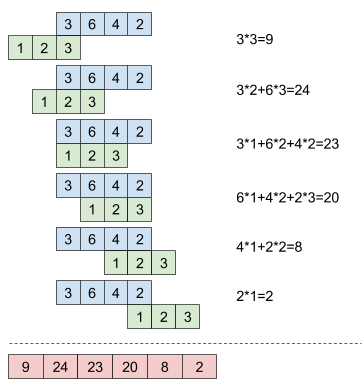
\includegraphics{cap2_ex_corr_cruz_1d.png}
	\caption[Exemplo de correlação cruzada 1D]{
		Exemplo de correlação cruzada 1D.
		Na imagem está sendo calculada a correlação cruzada entre $[3,6,4,2]$ e
		$[1,2,3]$. O primeiro conjunto de dados fica fixo enquanto o segundo vai
		sendo deslocado, e após cada passo se calcula a soma do produto, conforme
		ilustrado. O resultando é $[9,24,23,20,8,2]$. Todos os vetores
		representados possuem uma quantidade infinita de zeros à direita e à
		esquerda (autoria própria).}
	\label{fig:cap2_ex_corr_cruz_1d}
\end{figure}

A correlação cruzada também é definida para dimensões maiores que 1.
Tomando as funções discretas $f[n_1,n_2]$ e $g[n_1,n_2]$ pode-se 
escrever a convolução 2D destas funções como sendo:

\begin{equation}
	def: (f \star\star g)[n_1,n_2] =
		\sum_{m_1=-\infty}^{\infty} \quad
		\sum_{m_2=-\infty}^{\infty}
		f^*[m_1,m_2]g[m_1+n_1,m_2+n_2]
\end{equation}

É possível realizar convoluções para um número arbitrário de dimensões através
da generalização desta equação.

A aplicação do operador de correlação cruzado é próximo ao conceito de filtro
linear, bastante usado em processamento digital de imagens
\cite{gonzalezwoods200708}. Os conceitos não
são idênticos porque filtro digital trata uma das entradas como sendo
``sinal'',
e a outra como sendo o filtro, ou \emph{kernel}, e convoluções e correlações
cruzadas tratam as duas entradas de forma idêntica, e produzem um resultado
diferente nos extremos. Como observa-se na figura
\ref{fig:cap2_ex_corr_cruz_1d}, a saída é um vetor de dimensão 6, e um filtro
digital geraria saída de tamanho 4 (se houvesse extensão de borda).
No entanto, os números obtidos pelo filtro linear são iguais aos obtidos pela
correlação cruzada nas posições centrais. Mais detalhes sobre isso
serão cobertos na seção \ref{ses:bordas}.

A correlação cruzada entre $f[n]$ e $g[n]$
é igual à convolução entre $f[n]$ e $g[-n]$, e relações semelhantes existem
para qualquer dimensionalidade. Uma camada de uma rede
neural que use qualquer uma das operações é denominada “convolucional”,
pois neste contexto as operações são intercambiáveis. Ao se trocar convolução
por correlação
cruzada os mesmos parâmetros serão aprendidos em uma ordem diferente.
Por este motivo os termos ``convolução'' e ``convolucional'' são usados de forma
relaxada no contexto de redes neurais. Conforme será visto adiante, existe
mais um motivo para isso.

O uso de convoluções em redes neurais, especialmente para dimensões superiores
a 1, requerem que os dados nos quais este operador vai ser executado sejam
representados de forma a preservar a geometria original. Se os dados forem uma
imagem bidimensional, por exemplo, essa característica precisa ser preservada,
e a rede neural precisa conhecer a forma dos dados.

Uma das formas de estruturar os dados é usando tensores, que são uma
extensão de
vetores que admite um número arbitrário de dimensões. O motivo para isso é
permitir preservar a geometria da informação que está sendo processada.

Se a rede neural convolucional for aplicada em uma
imagem bidimensional com dimensões $H$ e $W$ com C canais de cor, ela pode ser
representada por um tensor de dimensões $H \times W \times C$. Uma imagem
tridimensional com profundidade $D$ é representada por um tensor
$D \times H \times W \times C$, e assim por
diante. Isso permite preservar o posicionamento relativo das informações
e viabiliza aplicar o operador de correlação cruzada.

Caso a rede neural esteja operando sobre um tipo de informação que não possui o
conceito de “canal”, como séries temporais, é conveniente artificialmente
criá-lo. Esse é o caso de séries temporais com “N” entradas, que serão
representadas por um tensor com dimensões $N\times1$. O motivo para isso é
uniformidade, como será explicado adiante.

\subsection{Camadas convolucionais}
Uma camada convolucional é definida pela a aplicação de um \emph{kernel} sobre
a sua entrada usando o operador convolução. Como já foi mencionado,
o uso do termo convolução
é bastante relaxado neste caso por que, além de normalmente referir-se a
uma correlação cruzada, é aplicado de forma idêntica à aplicação de um filtro
digital, gerando as diferenças já discutidas no resultado desta operação.

O filtro da camada convolucional é um tensor que contém parâmetros treináveis.
Se a entrada da camada convolucional tem dimensões
$D0 \times D1 \times D2 \times ... \times C$, onde C é o número de canais,
o filtro terá o mesmo número de dimensões, sendo que o tamanho de todas
as dimensões, exceto a última são
hiperparâmetros arbitrários. A última dimensão do filtro precisa ser igual ao
número de canais da imagem de entrada da camada convolucional, como ilustrado na
figura \ref{fig:ex_conv_2d}.


\begin{figure}[!htb]
	\centering
	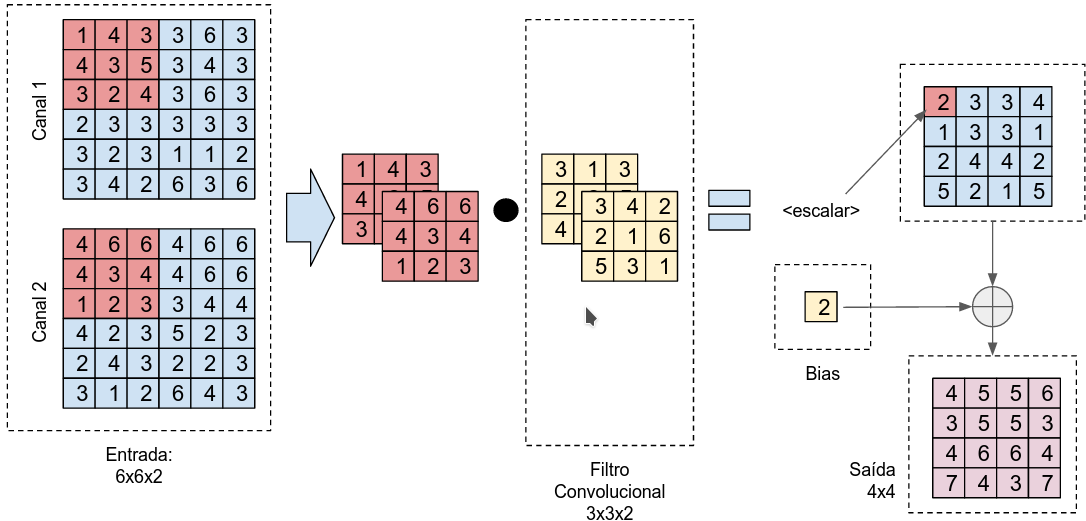
\includegraphics[scale=0.55]{ex_conv_2d.png}
	\caption[Exemplo de convolução 2D]{
		Exemplo de convolução 2D.
		Exemplo da aplicação de uma única convolução a uma imagem de
		entrada $6 \times 6 \times 2$. O tamanho da última dimensão do filtro e
		da entrada precisam ser iguais, no caso 2. As dimensões $3 \times 3$ do
		filtro foram escolhidas arbitrariamente. O símbolo do círculo na imagem
		representa um produto interno. A imagem de saída foi gerada deslocando
		a seleção de \emph{pixel} a \emph{pixel} até cobrir toda a
		imagem de entrada. Como as bordas não foram estendidas, a imagem
		resultante é menor que a de entrada (autoria própria).}
	\label{fig:ex_conv_2d}
\end{figure}

Camadas convolucionais também usam \emph{bias}, porém em uma quantidade muito
menor que as redes neurais totalmente conectadas. Se uma camada totalmente
conectada possui 100 neurônio ela vai ter 100 \emph{bias}. No caso de uma camada
convolucional, porém usa-se um único \emph{bias} por convolução. Na figura
\ref{fig:ex_conv_2d} existe apenas um bias, com o qual todos os valores da
saída serão somados.

\subsection{Bordas} \label{ses:bordas}
Como já foi mencionado, a convolução é aplicada de forma idêntica
a um filtro linear \cite{gonzalezwoods200708}, e assim como no caso dos
filtros lineares, existem algumas opções para tratamento de bordas dos dados.

Na figura \ref{fig:ex_conv_2d} o tamanho do tensor de saída foi reduzido
de 6 para 4. Neste caso a opção foi por não estender as bordas. Por
este motivo, o resultado tem que ser reduzido para impedir que o filtro
possua termos despareados.

Pode ser
desejável fazer a saída ter o mesmo tamanho da entrada. Para isso é necessário
estender as bordas da entrada, o que permitiria ao filtro ser deslocado por
toda a extensão entrada. Em camadas convolucionais observou-se apenas a
extensão com zeros. O software que foi adotado para a implementação deste
trabalho não suporta extensão que não seja com zeros, e não foi encontrado
artigo usando método diferente, como repetição.

A opção de extensão de borda é um hiperparâmetro.

\subsection{\emph{Stride}}
Ao se aplicar o filtro de convolução no tensor de entrada pode-se movê-lo de
posição a posição, até cobrir todos os locais válidos em cada direção, como
ilustrado na figura \ref{fig:ex_conv_2d}, ou pode-se desejar aplicar a cada
``$n_0$'' \emph{pixels} em uma direção, ``$n_1$'' \emph{pixels} em outra
direção, e assim por diante.  Esta opção é denominada \emph{stride}.

Quando uma camada convolucional possui como entrada um tensor de dimensões
$d1\times d2 \times ... \times dj \times C$, o \emph{stride} é definido como
sendo um tensor unidimensional de tamanho j.
O \emph{stride} $[1,2,1]$, por exemplo, indica que na primeira dimensão o
filtro será aplicado em todas as posições válidas, na segunda dimensão será
aplicado a cada 2 \emph{pixels} e na terceira será aplicada novamente em
todas as posições válidas. \emph{Stride} maior que 1 causa redução no
tamanho do tensor de saída.

Se um \emph{stride} $2 \times 2$ fosse aplicado na convolução da figura
\ref{fig:ex_conv_2d} a imagem de saída seria $2 \times 2$.

\subsection{Profundidade do Filtro}
A figura \ref{fig:ex_conv_2d} mostrou um único filtro sendo aplicado ao
tensor de entrada. No entanto, é possível aplicar um número arbitrário
deles, sendo que cada filtro produz um tensor de saída. O número de filtros é
denominado ``profundidade'' da camada convolucional.

A camada convolucional vai produzir uma saída para cada filtro. É conveniente
agrupar todas as saídas em um único tensor. Se a entrada da convolução
possui dimensões $d0 \times d1 \times ... \times C$ e a profundidade da camada
convolucional é $D$ pode-se representar as $D$ saídas com um tensor de
dimensões $d0 \times d1 \times ... \times D$. Observar que o tensor de saída
agora é semelhante ao tensor de entrada, substituindo apenas $C$ no tensor de
entrada por $D$ no tensor de saída. Se houver uma camada convolucional depois
desta ela vai tratar a última dimensão da mesma forma que esta trata o canal, o
que é conveniente. Se na figura \ref{fig:ex_conv_2d} fossem aplicados 8
filtros a saída seria um tensor $4 \times 4 \times 8$.

O tensor que representa o filtro também precisa receber uma dimensão adicional,
para poder representar todos os $D$ filtros, e também vai ser a última dimensão
do tensor. Sendo assim, para aplicar em uma imagem RGB 8 filtros $5 \times 5$ o
tensor que representa os pesos das convoluções possui dimensões $5 \times 5
\times 3 \times 8$.

\subsection{Processamento em Lotes}
Durante o treinamento das redes convolucionais o otimizador vai fazer
alterações nos valores dos parâmetros treináveis e precisa determinar se elas
melhoraram ou pioraram o desempenho. No caso de treinamento supervisionado
a rede neural é alimentada com dados e o resultado da classificação é comparado
com o valor esperado. É conveniente usar múltiplas imagens para este teste,
para que ele seja o mais representativo possível.

O número de imagens fornecidas é denominado ``tamanho do lote''. Se uma rede
neural trabalha com dados de dimensões $d0 \times d1 \times ... \times C$
podem-se agrupar $B$ exemplos em
um único tensor, com dimensões $B \times d0 \times d1 \times ... \times C$.
As camadas convolucionais tratam cada uma das imagens separadamente,
conforme já foi descrito, e emitem na sua saída um
único tensor com dimensões $B \times d0 \times d1 \times ... \times D$, sendo
$D$ a profundidade da camada. A figura \ref{fig:cap2_conv_block} ilustra as
entradas e saídas de uma camada convolucional usando lotes e profundidade.

\begin{figure}[!htb]
	\centering
	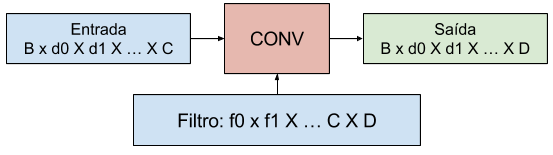
\includegraphics[scale=0.7]{cap2_conv_block.png}
	\caption[Convolução com múltiplos filtros e entrada em lote]{
		Convolução com múltiplos filtros e entrada em lote.
		Diagrama de uma camada convolucional de profundidade $D$ sendo aplicada em
		um lote contendo $B$ imagens. Ilustração não inclui \emph{bias}
		(autoria própria).}
	\label{fig:cap2_conv_block}
\end{figure}

\subsection{Pooling}
Após a aplicação de uma camada convolucional pode-se aplicar uma camada de
\emph{pooling}, que é uma forma de subamostragem. A figura
\ref{fig:ex_maxpool} ilustra um dos tipos de \emph{pooling}, denominado
\emph{maxpool}.

\begin{figure}[!htb]
	\centering
	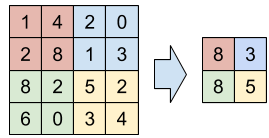
\includegraphics[scale=0.9]{ex_maxpool.png}
	\caption[Exemplo de \emph{maxpool} $2 \times 2$]{
		Exemplo de \emph{maxpool} $2 \times 2$ aplicado usando
		\emph{stride} $2 \times 2$. O filtro move de dois em dois \emph{pixels}
		e possui tamanho 2 em cada dimensão (autoria própria).}
	\label{fig:ex_maxpool}
\end{figure}

Esta operação possui como parâmetros o tamanho do filtro, o \emph{stride} e
a opção de
borda. A operação a ser aplicada no filtro pode ser $max$ ou $avg$ (média),
que definem respectivamente os filtros \emph{maxpool} e \emph{avgpool}.

Como as operações de \emph{pooling} são normalmente feitas com \emph{stride}
maior que 1 elas
acabam reduzindo consideravelmente o tamanho do tensor de saída. No caso de um
\emph{maxpool} $2 \times 2$, por exemplo, o tensor resultante vai ter 25\% do
número de valores do tensor de entrada.

Uma camada convolucional com \emph{pooling} pode ser contada como uma única
camada ou
como duas, dependendo do caso. Em algumas arquiteturas mais complexas, como em
\cite{szegedy2015going}, onde definem-se camadas do tipo \emph{inception},
pode não ser possível associar uma operação de \emph{pooling} a uma única
convolução, requerendo contagem separada.

\subsection{ReLu}
Assim como em redes neurais totalmente conectadas, pode-se aplicar uma função
de ativação para tornar a camada não-linear. As funções tangente
hiperbólica, sigmoide ou outras tipicamente usadas em redes neurais
não-convolucionais podem ser aplicadas. No entanto a função
\sigla{ReLu}{\emph{Rectified Linear Unit}, unidade linear retificada}, ou
linear retificada, resulta em treinamento substancialmente mais rápido enquanto
mantém a capacidade de generalização da rede neural treinada. A função
ReLu é definida por:


\begin{equation}
	ReLu(x) = max(0,x)
\end{equation}

Quando uma camada de uma rede neural inclui apenas elementos lineares,
ela é dita linear. O operador de convolução em si é linear, então
isso vai ocorrer quando a camada não inclui uma função de ativação, como
a ReLu e não possui outros elementos não-lineares, como \emph{maxpool},
caso o \emph{pooling} esteja sendo considerado como parte da camada
convolucional.

\subsection{Últimas Camadas}
Após as camadas convolucionais terem sido aplicadas é necessário usar um
classificador, mecanismo de regressão ou outro sistema que gere o tipo de saída
desejada para a rede neural. Uma das possíveis formas de realizar esta função é
usar uma ou duas camadas totalmente conectadas, como ilustrado na figura
\ref{fig:ex_cnn}. No exemplo a função de ativação da penúltima camada é
ReLu e a última camada é linear.

\subsection{Rede Neural Convolucional Completa}
Para alguns casos simples, pode-se construir uma rede neural convolucional
conectando-se uma camada convolucional a uma \emph{maxpool} e uma ReLu. Este
conjunto pode ser repetido algumas vezes até que o número de saídas da camada
convolucional seja baixo o suficiente para que seja passado por duas camadas
totalmente conectadas. Se houver interesse em não reduzir o tamanho total do
tensor pode-se omitir a camada \emph{maxpool}. Um exemplo dessa topologia é
mostrado na a figura \ref{fig:ex_cnn}.

A primeira camada da rede neural vai ter filtros que serão sensíveis a
características simples da entrada, que no caso de imagens seriam, por exemplo,
gradientes e trechos de linhas. Em
cada camada seguinte estas características são recombinadas com as detectadas
nas regiões vizinhas, formando conceitos progressivamente mais sofisticados a
respeito da imagem.

A topologia da rede neural e o conjunto de todos os hiperparâmetros definem o
número de parâmetros treináveis que a rede neural vai possuir e quantas
operações são necessárias para aplicar a rede neural em um (ou um lote de)
amostras. Uma rede neural mais larga, com um maior número de filtros por
camadas, possui a capacidade de aprender mais características. Redes neurais
mais profundas possuem capacidade de abstração maior, sendo capazes de inferir
a partir dos dados de entrada conceitos mais complexos. Se a rede neural for
mais complexa do que o necessário pode haver \emph{overfitting}.

\begin{figure}[!htb]
	\centering
	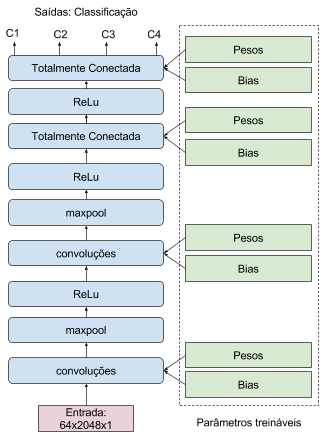
\includegraphics[scale=1]{ex_cnn.png}
	\caption[Exemplo de rede neural convolucional completa]{
		Exemplo de rede neural convolucional completa.
		Esta rede neural possui nove camadas para
		classificação de séries temporais em uma de 4 classes. Destacam-se os
		parâmetros treináveis (autoria própria).}
	\label{fig:ex_cnn}
\end{figure}

\subsection{Treinamento}
O treinamento de redes neurais convolucionais é feito de forma idêntica ao
treinamento de redes não-convolucionais. Para o caso de treinamento
supervisionado é necessário que se tenha acesso de exemplos rotulados.
Cada exemplo é formado por duas partes: entrada e saída esperada.
A entrada é denominada $x$, e é o conjunto de todos os valores que serão
fornecidos para a rede neural.
A saída esperada, denominada $y$, é o que se espera obter da rede neural.
Quando a entrada $x$ é fornecida para a rede neural ela vai produzir uma saída,
denominada saída estimada, ou $\widehat{y}$.

A rede neural possui parâmetros denominados hiperparâmetros e parâmetros
treináveis. O primeiro define características que são escolhidas manualmente
por quem está fazendo o treinamento. Isso envolve, entre outras coisas, o
número de camadas, e a quantidade de camadas. Pode-se dizer que a própria
escolha do método de classificação, como CNN ou HOG+SVM é um hiperparâmetro. Os
parâmetros treináveis são aqueles que são encontrados pelo processo de
treinamento.

O treinamento ocorre guiado por um valor denominado perda da rede neural, ou
\emph{loss}. A perda é um escalar real que mede o desempenho da rede neural.
Não importa quantas saídas a rede neural possui, ela vai sempre ter um único
real que representa a perda. Existem várias formas de se calcular este valor,
dependendo do uso da rede neural. Quando a rede neural faz regressão é comum o
uso da função de perda L2:

\begin{equation}
	\text{L2 loss}=
		\frac{1}{N} \sqrt{ \sum_{n=1}^N \left( y_n - \widehat{y}_n \right)^2 }
\end{equation}

Onde a raiz quadrada normalmente não é calculada, e algumas vezes usa-se a soma
ao invés da média. Também usa-se a perda L1, que é a média do módulo da
diferença entre os valores estimados e os esperados, e para classificação
usa-se a perda logística, ou entropia cruzada \cite{robert2014machine}.

O treinamento é realizado por um ``otimizador'', cujo papel é atualizar os
parâmetros treináveis para minimizar a perda. Os otimizadores mais usados são
derivados do \emph{gradient descent}, sendo \citeonline{kingma2014adam} um dos
melhores disponíveis.

Como otimizador depende da função de perda para atualizar os parâmetros da rede
neural, este valor precisa o mais representativo possível. Por isso ele deve
ser calculado em função de vários exemplos, não apenas um.

Durante o processo de treinamento um conjunto de exemplos vai ser usado e os
pesos vão ser atualizados uma vez, então um conjunto diferente de dados vai ser
usado para a interação seguinte. É importante que os exemplos estejam bem
embaralhados e contenham quantidades próximas de exemplos dos diversos tipos
que a rede neural vai processar. Se a rede neural estiver classificando imagens
em dois grupos $A1$ e $A2$, por exemplo, e todos os exemplos de uma classe
vierem depois da outra o treinamento não vai funcionar. Idealmente, a cada
interação do otimizador deve haver exemplos dos dois tipos.

%Eu acho que você fez um bom trabalho descrevendo como as CNNs são. Não tinha
%notado na versão anterior, mas nesta versão eu de repente senti falta de pelo
%menos uma menção ao treinamento.
%
%Minha sugestão: coloque uma última sub-seção antes da 2.3, e fale BREVEMENTE
%sobre o treinamento. Eu sei que se você tentar explicar a fundo, vai ficar
%grande e complicado demais. Do ponto de vista do SEU trabalho, entender COMO
%uma CNN é e como USAR ela é (muito) mais importante do que o algoritmo de
%treinamento. Tendo isso em mente, você pode ser bem breve, é coisa de menos de
%meia página.

\section{Uso em Processamento de Imagens}
O uso de redes neurais convolucionais é uma alternativa a diversos métodos já
existentes de detecção e reconhecimento de objetos em imagens. Aqui serão
mostradas algumas das alternativas usuais, para que sejam contrastadas
com a classificação baseada em redes neurais convolucionais.

\subsection{Redes Neurais Não-Convolucionais}
Quando uma imagem vai ser processada por uma rede não-convolucional ela precisa
ser convertida para a forma plana, em um vetor com dimensões
$H \cdot W \cdot C \times 1$.

O uso de camadas totalmente conectadas é proibitivo para classificação de
imagens desta maneira. Se uma rede neural for usada para processar imagens de 1
\emph{megapixel}, ou $720 \times 1280$, e a primeira camada possuir um
número de neurônios igual
ao número de neurônios da camada de entrada, a matriz de pesos teria
$(720 \cdot 1280 \cdot 3)^2 \approx 7.6 \cdot 10^{12}$ parâmetros. Se for
representado por números ponto-flutuante de 32 bits isso ocuparia mais de
30 TiB. O mesmo processo em uma imagem 480px por 640px geraria quase 850
bilhões de parâmetros só na matriz de pesos.

Outras topologias mais esparsas podem ser construídas, mas este tipo de rede
neural possui outros problemas que as tornam inviáveis para processamento direto
de imagens. Um exemplo é o fato delas não serem invariantes ao deslocamento. Se
a rede neural aprende a reconhecer um \emph{feature} em um local da
imagem, não vai
conseguir reaproveitar essa capacidade em outras posições. Portanto teria que
aprender a mesma \emph{feature} em cada possível posição onde ela possa
aparecer, e fazer isso para todas as \emph{features}.

Como a primeira operação feita foi converter a imagem para um formato “plano”, a
geometria da imagem foi destruída. Não é mais possível determinar quando dois
\emph{pixels} estão próximos, e essa é uma informação muito importante sobre a
imagem.

\subsection{Uso de descritores}
Uma das abordagens possíveis para reconhecimento e detecção de imagens é o uso
de descritores. Descritores são operações que tomam uma imagem como entrada e
resumem as sua
características em um conjunto menor de informações. Exemplos de descritores muito
usados são
\sigla{LBP}{\emph{Local binary patterns}, padrões binários locais}
	\cite{wang1990texture},
\sigla{ORB}{\emph{Oriented FAST and rotated BRIEF}, FAST orientado e BRIEF
	rotacionado} \cite{rublee2011orb},
\sigla{HOG}{\emph{Histogram of oriented gradients}, histograma de gradientes
	orientados} \cite{dalal2005histograms},
Haar-Wavelets \cite{nabout2008object},
filtros de Gabor \cite{riaz2012invariant}.
O treinamento é realizado sobre
as \emph{features} extraídas pelo descritor escolhido usando um
classificador como redes neurais ou \sigla{SVM}{\emph{Support Vector Machine},
	máquinas de vetores de suporte} \cite{boser1992training}
	\cite{cortes1995support}.

Para usar esta abordagem um descritor precisa ser escolhido e configurado,
muitas vezes manualmente. O desempenho do sistema como um todo vai depender
dessas escolhas. Se a operação de detecção depender de conceitos complexos,
envolvendo correlação entre múltiplas características, o descritor e o
classificador precisam ser escolhidos especificamente para isso.

\subsection{Redes Neurais Convolucionais em Imagens}
As redes neurais convolucionais operam diretamente nos \emph{pixels} da imagem,
não sendo necessário escolher um descritor, e não possuem os problemas que as
redes não-convolucionais possuem. As camadas convolucionais se comportam como
descritores, porém os parâmetros são aprendidos como parte do processo de
treinamento, portanto são otimizados para responderem precisamente para os
exemplos que forem fornecidos. Apenas alguns hiperparâmetros, como tamanho
da convolução, número de filtros e de camadas precisam ser escolhidos mediante
decisões de meta de precisão e \emph{recall}, tempo para classificação e
complexidade dos conceitos a serem aprendidos.

Para que seja possível usar convoluções é preciso preservar a
geometria dos dados. Se uma imagem de 40
\emph{pixels} de altura por 120 \emph{pixels} de largura contendo 3 canais de
cor for usado na
entrada de uma rede neural convolucional, ela precisa ser representada por um
tensor apropriado, como $32 \times 40 \times 120 \times 3$. Este tensor
permite alimentar a rede neural com um lote de 32 imagens.

Para aplicar uma camada convolucional à imagem de entrada escolhe-se o tamanho
da convolução, o número de filtros e o modo de operação nas bordas. A figura
\ref{fig:ex_cnn_img} ilustra um filtro $3 \times 3$ sendo aplicado a uma imagem
\sigla{RGB}{\emph{Red, green, blue}, vermelho, verde, vermelho}.
Para que o filtro tenha profundidade 64, por exemplo, o tensor que define o
filtro será $3 \times 3 \times 3 \times 64$ e o tensor resultante da
convolução será $32 \times 40 \times 120 \times 64$,
considerando que seja usado preenchimento nas bordas.

\begin{figure}[!htb]
	\centering
	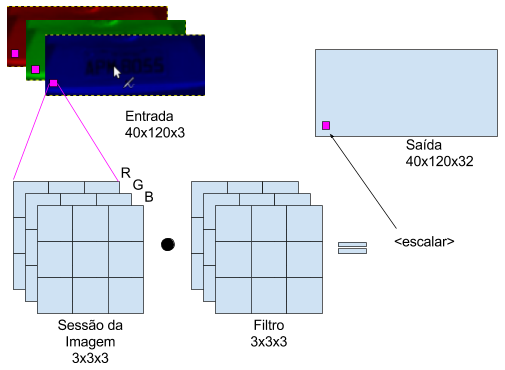
\includegraphics[scale=.8]{ex_cnn_img.png}
	\caption[Convolução sendo aplicada em uma imagem RGB]{
		Convolução sendo aplicada em uma imagem RGB.
		Como a imagem possui 3 canais o filtro será $3 \times 3 \times 3$.
		Uma partição da imagem original com o mesmo tamanho do filtro,
		$3 \times 3 \times 3$ é extraída da imagem, e um
		produto interno é realizado entre os dois, resultando em um escalar. Este
		escalar é armazenado no tensor de saída nas coordenadas corretas. A
		ilustração só mostra uma imagem de entrada e só um filtro e, portanto, uma
		imagem de saída (autoria própria).}
	\label{fig:ex_cnn_img}
\end{figure}

Para finalizar a camada convolucional adiciona-se um \emph{bias}. Para
isso usa-se um escalar para cada uma das 64 imagens resultantes. O
tensor que define os \emph{bias} é um tensor unidimensional com tamanho 64.

Camadas \emph{maxpool} e ReLu podem ser adicionadas para reduzir as
dimensões da imagem ou aumentar a sua não-linearidade. A figura
\ref{fig:ex_full_cnn_img} ilustra o uso das três camadas em sequência.

\begin{figure}[!htb]
	\centering
	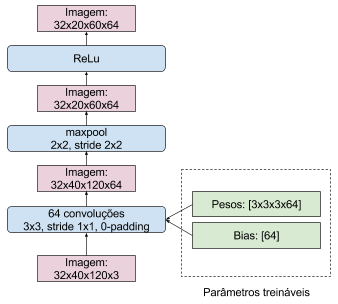
\includegraphics[scale=1.2]{ex_full_cnn_img.png}
	\caption[Exemplo de rede neural convolucional completa aplicada à uma imagem
		RGB]{
		Exemplo de rede neural convolucional completa aplicada à uma imagem
		RGB.
		Uma sequência de operações é realizada usando uma rede neural
		convolucional incluindo 64 convoluções $3 \times 3$, \emph{maxpool} e
		ReLu aplicadas em um
		lote de 32 imagens $40 \times 120 \times 3$. Os parâmetros treináveis
		estão destacados (autoria própria).}
	\label{fig:ex_full_cnn_img}
\end{figure}

A imagem é tratada por camadas sucessivas de convolução, \emph{maxpool} e
ReLu até que
o tamanho total do tensor seja pequeno o suficiente para poder ser processado
por duas camadas totalmente conectadas. 

\subsection{Uso de Cores}
Em alguns sistemas de visão computacional são usadas imagens em
tons de cinza. No caso de redes convolucionais o mais comum é usar
imagens coloridas.
O primeiro motivo para isso é que as imagens e vídeos são normalmente
captadas com cores, então o processo de detecção teria que incluir uma operação
de conversão para escala de cinza. 

Pode-se demonstrar que todos os métodos de conversão lineares de RGB para
escala de cinzas, como:

\begin{equation} \label{eq:rgb2gray}
	C=0.299R + 0,587G + 0.114B
\end{equation}

podem ser representados como uma convolução $1 \times 1$. Visto que as
convoluções são implementadas de forma bastante eficiente nas bibliotecas
de redes neurais convolucionais, algumas vezes até usando aceleração por
hardware, não necessariamente haverá economia durante a execução
durante a execução da rede neural. No pior caso, quando a cor não
é útil, a CNN pode fazer
essa conversão de forma eficiente, sendo que os coeficientes associados
a cada canal, que no exemplo da equação \ref{eq:rgb2gray} são fixos, podem
escolhidos pelo otimizador, potencialmente obtendo uma conversão mais
apropriada para o caso específico onde a rede neural está sendo aplicada.

Outro ponto é que os sistemas que representam o atual
estado-da-arte para reconhecimento de imagem, como \cite{szegedy2015going}
\cite{hasanpour2016lets}, usam cores, portanto nos casos onde
existe \emph{budget} computacional, e particularmente quando é possível usar
vários filtros convolucionais na primeira camada, a informação da cor pode
ser vantajosa para minimizar os erros da rede neural.

\subsection{Reconhecimento de Objetos}
Existem várias maneiras de se usar redes neurais para reconhecer objetos. Duas
das opções envolvem configurar a rede neural como classificador e como
sistema de regressão.

Para usar a rede como classificador pode-se incluir na última camada da rede
neural um sistema \emph{softmax}, também conhecido como exponencial
normalizada. Isso
permite que a rede neural seja treinada e, após o treinamento, estime a
probabilidade da sua entrada pertencer a cada uma de N classes. A rede neural é
implementada usando $N$ saídas, de forma que cada saída é treinada para
representar a probabilidade da entrada ser classificada em uma das classes.
Uma camada \emph{softmax} realiza uma normalização das saídas da rede neural,
usando a equação:

\begin{equation}
	softmax[i] = \frac
		{exp\left( \widehat{out}[i] \right)}
		{\sum_j exp\left( \widehat{out}[j] \right)}
\end{equation}

Para identificar a presença ou não do objeto que está sendo procurado, duas
classes seriam definidas: ``presente'' e ``não-presente'', resultando em uma rede
neural como mostrada na figura \ref{fig:ex_classif_logist}.

\begin{figure}[!htb]
	\centering
	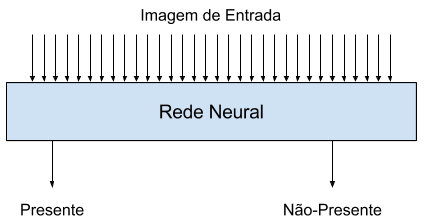
\includegraphics[scale=0.8]{ex_classif_logist.png}
	\caption[Exemplo de Classificador Logístico]{
		Exemplo de Classificador Logístico.
		Este exemplo de rede neural possui uma imagem como entrada e possui duas
		saídas, uma informando a probabilidade da imagem conter o objeto, outra
		indicando a probabilidade de não conter (autoria própria).}
	\label{fig:ex_classif_logist}
\end{figure}

Este modelo pode ser treinado usando modo supervisionado, onde imagens
pré-classificadas são fornecidas. A função de perda a ser minimizada pelo
otimizador é a função \emph{cross entropy}:

\begin{equation}
	\widehat{H} = - \sum_i \widehat{y_i} log(y_i)
\end{equation}

Onde $y_i$ é o valor da probabilidade manualmente
marcada de uma imagem pertencer à classe $i$ (no caso, a probabilidade de ser
uma imagem que contém o objeto e a probabilidade de não conter) e $\widehat{y_i}$
é o valor estimado pela rede neural. $\widehat{H}$ é o valor estimado de
\emph{cross entropy}.

Quando tem-se o objeto desejado centrado na imagem a saída ``presente`` deve
ser 1 e a outra saída 0. Quando o objeto não é visível em lugar nenhum no campo
visual da rede neural os valores devem ser invertidos.
Os casos onde o objeto está visível apenas parcialmente devem ser considerados
cuidadosamente, produzindo valores intermediários nos rótulos, para evitar que
duas imagens parecidas gerem valores muito diferentes na saída da rede neural.

As redes neurais também podem ser usadas para fazer regressão, ou seja, modelar
uma função. Uma forma usual de implementação é a regressão L2. Neste tipo de
função o otimizador vai minimizar o erro quadrático:

\begin{equation}
	E=sum \left( \left( y - \widehat{y} \right)^2 \right)
\end{equation}

Sendo que $sum$ é uma função que representa a soma de todos os valores do
tensor que recebe como parâmetro.
A rede neural pode ser usada para modelar a função $P$, definida por:

\begin{equation}
	y = P(img) = \begin{cases}
		1 \text{, se img contém o objeto procurado} \\
		t(img) \text{, se objeto está parcialmente visível} \\
		0 \text{, se img não contém}
	\end{cases}
\end{equation}

Detectores podem encontrar o objeto que estão procurando parcialmente presentes 
no seu campo de visão, e esta função precisa tratar desta possibilidade. No
caso, a condição de transição, representada por $t(img)$, não está sendo
aqui definida, pois cada implementação deve escolher esta função cuidadosamente
para integração com o \emph{software} que vem depois da rede neural.
Uma coisa que não pode ocorrer é descontinuidade entre duas imagens próximas,
especialmente no caso de translação, pois o otimizador teria que encontrar
pesos que modelassem a descontinuidade, e mesmo uma pequena imprecisão nestes
pesos vai gerar um erro muito grande.

\subsection{Localização de Objetos} \label{sec:localiz_objetos}
Até agora foi mostrado como usar redes neurais convolucionais para detectar um
objeto em uma imagem. Isso envolve apenas determinar se uma imagem possui ou não
o objeto de interesse. Localização, ao contrário, requer a determinação das
coordenadas do objeto. Em alguns casos pode requerer o cálculo do retângulo
envolvente mínimo ou até da curva de perímetro do objeto.

Um sistema de localização pode ser construído a partir de um sistema de
detecção. A abordagem mais simples para isso envolve construir um sistema capaz
de detectar o objeto de interesse e aplicar este
detector à imagem várias vezes a imagem usando ``janelas deslizantes''.
Se o detector for construído para produzir ``1'' quando detectar o objeto e
“0” caso contrário, então os pontos de máxima são candidatos a centros dos
objetos.

Se os objetos puderem variar muito em tamanho pode ser necessário o uso de
técnica de aplicação multi escala, onde a janela deslizante também é aplicada a
versões reduzidas da imagem. Caso o objeto procurado varie pouco em tamanho
isso não é necessário.

Como cada \emph{pixel} da imagem é candidato a centro do objeto que está sendo
localizado, deve-se aplicar o filtro uma vez para cada \emph{pixel}. Se não
houver extensão de bordas, o filtro não pode ser aplicado em parte dos
\emph{pixels}.

